\chapter{绪论}

\section{课题背景与研究意义}

依托以互联网为代表的信息技术的高速发展,我国社会当前正处在由传统服务业向现
代服务业全面升级的重要历史进程中。充分利用和结合现代先进的信息技术,提供信息和
知识更加密集、附加值更高的服务是现代服务业的基本要求。互联网作为现代信息服务的
载体,从早期简单的门户网站、搜索引擎,发展到社交网站、即时通信\cite{王晓玲2015我国现代服务业借力},再到移动搜索、LBS
等移动互联网应用的风靡,在产业规模持续扩大的同时,也不断向各行各业渗透,从早期
的传媒、游戏等行业,到娱乐、零售行业,再到金融、教育和医疗等行业,影响范围还在不
断继续扩大\cite{王晓玲2015我国现代服务业借力}。由此可见,未来服务的基础形态一定是基于互联网的,各行业通过互联网来
提供他们的服务是大势所趋。


% 跨界服务网络将跨越不同行业、组织、价值链等边界的服务进行深度融合和模式创新,为用户提供多维度、高质量、富价值的跨界服务,成为现代服务业发
% 展的重要创新途径。
跨界服务平台是各类跨界服务集成的支撑系统,相比传统的服务集成,跨界服务融合需开展模式、生态、环境、质量、价值等多维深度融合,
导致内部服务种类繁多、数量庞大,用户在进入系统后,面对如此数量的服务,很难快速检索到想要的服务,面向用户的服务检索以及如何提升用户体验成为问题。
随着人工智能的飞速发展,人机对话越来越受到人们的关注。人机对话系统主要由自动文本、语音识别,语义理解,对话内容管理,
对话内容生成和交互组成。在人机对话过程中,面向任务的对话最紧急的事情要做的是获取用户的真实意图。经过一轮或多轮对话后的上下文综合判断,
可以准确捕捉用户的意图并尽快完成面向任务的对话。
这其中最重要的一环是语义理解,直接影响到系统能否提取用户需求,语义理解可被分为领域分类、意图识别和语义槽填充三个子模块。
意图检测作为自然语言理解的一个子模块,在提高自然语言理解和口语理解方面起着至关重要的作用。
领域、意图检测设法捕获用户的真实意图和用户的期望动作,例如饭店预订,机票查询等。语义槽填充可视为序列标注,主要工作是实体提取,需要在语义层面更细粒度的理解。

借助人机对话的思想,本文在跨界服务平台中引入智能服务调用引擎,其核心是用户语义理解。用户进入平台以后,可以输入带有自己意图的语句,如“查询成都开往杭州的火车票”,
智能服务调用引擎接受语句以后进行语义理解,识别并找出系统内部与之匹配的服务,从句子中提取参数完成调用返回结果,从而解决了用户检索服务困难的问题,
简化了用户操作,提升了用户体验,让系统更加智能化。本文着重研究了智能调用中的语义理解,语义理解是自然语言处理任务的重要基石,作用是使计算机能够对人类语言的结构和含义的理解,
从而允许用户使用自然语句与计算机进行交互。本文提出的文本分类和语义槽填充模型,不局限于跨界服务场景,对模型稍作修改,可应用于许多
其他的同类型任务中,如情感分析,内容分析,任务型对话系统等。本文将NLU技术应用于跨界服务领域,拓宽了自然语言处理技术的界限。

\begin{figure}[htbp]
  \centering
  
\includegraphics[scale=0.4]{./images/kuajiefuwu.png}
  \caption{跨界服务}
  \label{fig:kuajiefuwu}
\end{figure}


% 现代服务业是中国经济发展战略中的重要组成部分,也是衡量一个国家经济发展水平
% 的重要标志。推动现代服务业的发展壮大已成为当前中国经济发展的重要目标和关键动力\cite{唐任伍2012公共服务跨界合作}。
服务计算作为现代服务业发展的重要技术基础,需要结合现代服务业发展的具体场景和具体问题进行深入的研究和应用。
本文依托于国家重点研发计划专项的子课题《跨界服务集成方法与支撑载体》,围绕在研究跨界服务集
成和交互过程中发现的服务种类数量繁多用户检索困难、交互缺乏智能化的问题,在跨界服务平台中引入服务智能调用引擎并重点研究了其核心用户语义理解模型,
用户检索服务困难的问题,
简化了用户操作,提升了用户体验,让系统更加智能化。

综上所述,本文在跨界服务平台基于深度学习算法设计并实现了用户语义理解模型,跨界服务系统利用该模型提取分析用户输入的语句的语义,
在系统内部检索匹配服务自动执行返回结果展示,完成服务的智能化调用。

\section{国内外研究现状}
% \subsection{跨界服务}
% “云大物移智”等新一代信息技术的发展与应用,使得人类的认知扩大、能力增强,
% 也将重新定义传统边界。“跨界”即突破原有界限,实现界内和界外资源的整合与协作。
% 跨界服务将跨越不同行业、组织、价值链等边界的服务进行深度融合和模式创新,为用
% 户提供多维度、高质量、富价值服务,这不仅是技术发展的必然,也是现代服务业发展
% 的重要创新途径。

% 相比传统的服务集成,跨界服务融合需开展模式、生态、环境、质量、价值等多维
% 深度融合,具有极大挑战。目前国内外依然缺少跨界服务本质规模与模式认知、设计与
% 管理方法、质量管理与价值工程等方面的系统研究,也缺少相关工程方法和支撑载体。
% 从以下四个方面综述国内外的相关研究:

% (1) 服务模式创新是推动现代服务业快速发展的重要因素。近年来,国际上出现
% 了以Artifact 为中心的商业流程建模方法、基于商业交易过程的商业模式分析框架等,
% 对服务模式进行了分析和建模;国内浙江大学首次提出了跨界服务概念及其3C 特点。
% 但总体来看,目前学术界在跨界服务本质规律认知、模式定量分析与评估等方面仍处于
% 探索阶段。

% (2) 跨界服务设计关注如何获取和分析角色多元的用户真实需求,并根据用户需
% 求进行服务架构、流程和接口等生态设计。IBM 研究院、北京大学、武汉大学等单位的
% 研究团队在服务需求建模、服务设计和服务互操作性管理等方面具有较好的研究积累,
% 做出了一系列代表性工作如SOMA-ME、RGPS 需求元建模框架、基于Tropos 的服务建模
% 方法等,但针对跨界服务融合的设计目前仍缺少完整、系统的支撑方法体系。

% (3) 跨界服务融合需要高效、可靠的运行支撑环境,以提供服务网络的运行态支
% 持。目前这一领域主要有企业服务总线、企业应用集成等相关技术,北京大学、IBM、
% 佐治亚理工学院等在云端融合资源服务化、服务总线等方面具有较好研究积累,但这些
% 技术大多针对企业级运行环境,仅实现服务的结构和信息融合,难以应对跨界服务所需
% 的多维深度融合、动态服务网络优化、开放环境安全管控等挑战。

% (4)对服务系统进行精准的能力配置以提供特定的质量与价值,并在运行时准确
% 感知它们的实际提供水平以做出调控和改进。IBM 研究院、荷兰阿姆斯特丹自由大学、
% 哈尔滨工业大学等单位的研究团队在服务质量设计与度量、服务价值建模、服务价值感
% 知等方面具有较好的研究积累,做出了一系列代表性工作,如VASEM、服务价值网等,
% 但针对跨界服务质量体系和价值工程的研究仍处于初期阶段。

\subsection{文本分类}
文本分类任务是语义理解任务的重要组成部分,
文本分类是为给定的自然语言文本段自动分配预定义标签,选择标签以反映文本的“含义”。
文本分类应用在许多NLP任务中,例如情感分析,主题分类,问答系统和对话行为分类等。
文本分类方法可分为浅层学习模型和深度学习方法,
浅层文本分类模型一般首先利用手工手段得到较好的数据特征,之后利用传统的机器学习算法进行分类,所以此方法大大受限于第一步的特征提取。
然而与浅层文本分类模型不同,深度学习是一种端到端的实现进而将浅层模型利用人工的特征提取嵌入模型训练过程中。

\begin{figure}[htbp]
  \centering
  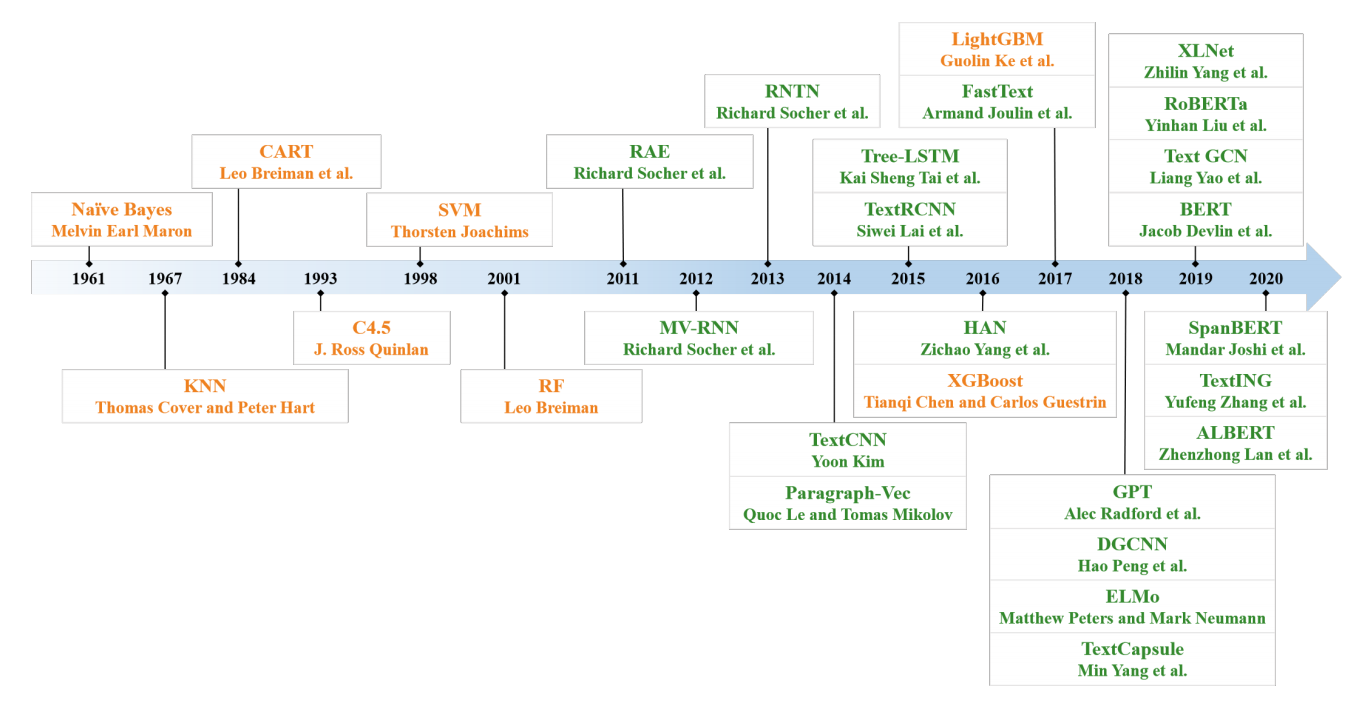
\includegraphics[width=16cm]{./images/text.png}
  \caption{文本分类技术研究发展趋势\cite{li2020survey}}
  \label{fig:textClassification}
\end{figure}

图\ref{fig:textClassification}为文本分类技术研究发展趋势,其中在2010年以前,文本分类模型主流算法为浅层学习。
在2010年以后,主流算法渐渐地从浅层学习模型转变为深层学习模型,
深度学习方法绕开了手工特征提取,利用数据驱动为文本提供了上下文相关的表示形式,
DNN根据数据集的特征,将单词向量输入到网络中进行训练,直到收敛为止。
文本分类任务中最受广泛使用的两种DNN方法是RNN和前馈神经网络,之后CNN和attention机制被引入进来,模型的性能达到新的高度,
目前最新的研究主要通过BERT和GNN来实现。

% 文本分类训练模型的性能由下游任务验证,例如情感分类,问题回答和事件预测。
% 前馈神经网络和递归神经网络是文本分类任务中使用最多的两种深度学习方法
% 渐渐的,CNN,RNN和注意力机制被用于文本分类,许多研究人员通过改进CNN,RNN和注意力机制,将模型融合和通过多任务方法来提高针对不同任务的文本分类性能。
% 可以生成上下文词向量的基于transformer的双向编码器BERT\cite{devlin2018bert}的出现,是文本分类和其他NLP技术发展的重要转折点。
% 许多研究人员已经提出了基于BERT的文本分类模型,该模型在包括文本分类在内的多个NLP任务中比上述模型具有更好的性能。
% 此外,一些研究人员研究了基于GNN的文本分类技术,以捕获文本中的结构信息,这是其他方法无法替代的。

2013年,Google开发了一系列word2vec模型\cite{mikolov2013distributed},这些模型接受了60亿个单词的训练,并立即在许多NLP任务中流行。 
2017年,来自AI2和华盛顿大学的团队开发了基于3层双向LSTM的上下文嵌入模型,称为ELMo\cite{peters2018deep},该模型比word2vec性能更好,因为它捕获了上下文信息。
在2018年,OpenAI开始使用Transformer\cite{vaswani2017attention}构建嵌入模型,Transformer是Google开发的一种新的NN架构,完全基于注意力,
从而大大提高了在TPU上进行大规模模型训练的效率,他们的第一个应用Transformer的模型称为GPT\cite{radford2018improving},现已广泛用于文本生成任务。
同年,谷歌开发了基于Transformer的BERT\cite{devlin2018bert},BERT由340M参数组成,经过33亿个单词的训练,是当前最先进的嵌入模型,
使用更大模型和更多训练数据的趋势仍在继续,OpenAI的最新GPT-3模型\cite{brown2020language}包含1700亿个参数,
而Google的GShard\cite{lepikhin2020gshard}包含6000亿个参数。
尽管这些巨大的模型在各种NLP任务上显示出了非常出色的性能,但一些研究人员认为它们并不真正理解语言,因此对于许多关键任务领域而言性能依然不够强大。
综上所述,可以根据其神经网络架构将DNN文本分类分为:递归神经网络(RNN),卷积神经网络(CNN),注意力,Transformer,胶囊网络等。


\subsection{命名实体识别}
参数提取(语义槽填充)任务可以视为命名实体识别(NER),NER的目标是提取给定文本中提及的命名实体,并将其分类为事先定义好的类别,
例如location,org,name等。
尽管早期基于统计规则的NER系统产生了不错的识别精度,但是需要精心设计规则和特征,因此通常需要大量的人工成本。
近年来,深度学习已被应用于NER系统中,并产生了优异的性能。

NER的演变过程,如图\ref{fig:nerp}所示。MUC-6会议上“命名实体”(NE)的概念首次被提出,
关于NER中应用的技术,按照时间顺序的主流方法有以下几种:

\begin{figure}[htbp]
  \centering
  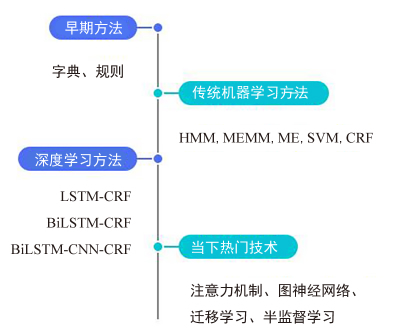
\includegraphics[scale=1]{./images/nerp.jpg}
  \caption{命名实体识别技术研究发展趋势\cite{nadeau2007survey}}
  \label{fig:nerp}
\end{figure}

(1)基于统计规则的方法

基于规则的NER系统依赖于人工手动制定的规则,可以基于特定领域的地名词典和句法词法模式设计规则。
Kim等提出使用布里尔规则推理方法进行语音输入,该系统会根据Brill的语音标记器自动生成规则\cite{kim2000rule},
在生物医学领域,Hanisch等提出了ProMiner,它利用预处理的同义词词典来识别生物医学文本中提及的蛋白质和潜在基因\cite{hanisch2005prominer}。 
% Quimbaya等提出了一种基于字典的电子健康记录中NER的方法,实验结果表明,该方法在对精度的影响有限的前提下可提高召回率。
其他一些基于规则的知名NER系统包括LaSIE-II,NetOwl,Facile,SAR,FASTUS和LTG等\cite{pomares2016named},
这些系统主要基于手工制定的语义和语法规则来识别实体,当词汇详尽无穷时,基于规则的系统可以很好地工作。
显然,此方法迁移到其他域会遇到很大的挑战,同时由于规则和词典的不完整性与局限性,NER系统常常会产生高准确率和低召回率的结果。

% (2)无监督学习方法

% 基于无监督的NER系统常用方法是聚类,

% 无监督学习的一种典型方法是聚类,基于聚类的NER系统根据上下文相似性从聚类类簇中提取命名实体,
% 其核心思想是,可以使用在大型语料库上计算出的词汇资源,词汇模式和统计信息来推断命名实体。 
% Collins等使用未标记的数据将对监督的要求减少到仅需7个简单的“种子”规则\cite{collins1999unsupervised},
% 并提出了两种用于命名实体分类的无监督算法。类似地,Etzioni等利用一组谓词名称作为输入,并利用一小组通用提取模式实现识别过程\cite{etzioni2005unsupervised}。 
% Nadeau等提出了一个非监督系统的地名词典建设和命名实体歧义解决方案,该系统基于简单而高效的启发式方法,结合了实体提取和歧义消除功能\cite{nadeau2006unsupervised}。
% 另外,Zhang和Elhadad提出了一种从生物医学文本中提取命名实体的无监督方法\cite{zhang2013unsupervised},
% 他们的模型求助于术语、语料库统计信息(例如逆文档频率和上下文向量)和浅层语法知识(例如名词短语分块),
% 在两个主流生物医学数据集上进行的实验证明了其无监督方法的有效性和可推广性。

(2)基于特征的监督学习方法

通过监督学习,NER被转换为多类别分类或序列标记任务。
对每一个待处理数据利用特征工程对输入进行模式转换,
之后使用机器学习算法训练模型,从未标注数据中识别出相似的模式,常用的方法
包括隐马尔可夫模型(HMM),决策树,最大熵模型,支持向量机(SVM)
和条件随机场(CRF)。Bikel等提出了第一个基于隐马尔可夫模型的NER系统,名为IdentiFinder,用于识别分类名称,
日期,时间表达式和数字\cite{bikel1998nymble,bikel1999algorithm}。此外,Szarvas等通过使用决策树和AdaBoostM1学习算法开发了一种多语言NER系统,
它可以训练几个独立的决策树分类器,然后通过表决方案组合进行决策\cite{szarvas2006multilingual}。 
Borthwick等通过应用最大熵理论提出了“最大熵命名实体”(MENE),MENE能够在做出标记决策时利用各种知识资源\cite{krishnan2006effective}。
 McNamee和Mayfield使用了1000种与语言相关的特征和258种拼字法和标点特征来训练SVM分类器,每个分类器都会做出决策,判断当前token是否属于既定的类别之一\cite{mcnamee2002entity}。
 在预测实体标签时,SVM没有考虑相邻词之间的联系,CRF则考虑了上下文\cite{mccallum2003early}。 
%  McCallum和Li提出了NER中CRF的特征归纳方法,在CoNLL03上进行了实验,成绩达到了84.04%。 
%  Krishnan和Manning提出了一种基于两个耦合CRF分类器的两阶段方法,第二个CRF利用从第一个CRF的输出中得到的潜在表示。

 (3)深度学习方法

 近年来,基于DL的NER模型逐渐占据主导地位,并取得了最优异的成果,与基于特征的方法相比,深度学习能够自动发现隐藏的特征。 
 将深度学习技术应用于NER有三个核心优势,首先,NER受益于非线性变换,该变换生成从输入到输出的非线性映射。
 与线性模型(对数线性HMM和线性链CRF)相比,基于DL的模型能够通过非线性激活函数从数据中学习复杂的特征。
 其次,深度学习为设计NER特诊节省了大量精力,传统的基于特征的方法需要大量的人力和领域专业知识,
 基于DL的模型可有效地从原始数据中自动学习有用的表示形式和潜在特征。
 第三,可以通过梯度下降在端到端模型中训练深度神经NER模型,此特性使能够设计复杂的NER系统。
 BiLSTM-CRF是使用深度学习的NER最常见的体系结构,
 以cloze-style方式预训练双向Transformer模型的方法在CoNLL03上实现了最优异的性能(93.5%)\cite{baevski2019cloze}。 
 Zhang 和 Yang 提出了一种针对中文NER的格子结构LSTM模型,该模型对输入字符序列以及与词典匹配的所有潜在单词进行编码\cite{zhang2018chinese}。

%  输入的分布式表示形式考虑了单词和字符级别的嵌入,现有的分类法基于字符级编码器,单词级编码器和标签解码器,以及结合了对功能有效的POS标签和地名词典等附加功能,
%  上下文编码器将使用CNN,RNN或其他网络捕获上下文相关性,标签解码器为输入序列中的token预测标签。
%  例如,在图\ref{fig:nerDL}中,每个token都被预测为带有其类型的命名实体:即带有B-(开头),I-(内部),E-(结束),S-(单个),或O-(外部)的命名实体。
%  当然,还有其他标记方案或标记符号,例如BIO。还可以训练标签解码器以检测实体边界,然后将检测到的文本跨度分类为实体类型。


% NER系统的成功很大程度上取决于其输入的表示形式,集成或微调预训练的语言模型嵌入正成为神经NER的研究热点,
% 利用这些语言模型嵌入时,可以显着提高性能。
% 我们从三个角度讨论利弊:输入,编码器和解码器。 
% 首先,关于是否应该使用外部知识或如何将其集成到基于DL的NER模型尚未达成共识,
% 一些研究表明,外部知识可以提高NER的表现。
% 但是,缺点也很明显:1)获得外部知识是劳动密集型的(例如地名词典)或计算上昂贵的(例如依赖项); 2)整合外部知识会对端到端学习产生不利影响,并损害基于DL的系统的通用性。
% 其次,当在大型语料库上对Transformer进行预训练时,Transformer编码器比LSTM更有效。如果未预先训练且训练数据有限,则Transformer将无法完成NER任务\cite{guo2019star,yan2019tener}。
% 第三,RNN和Pointer Network解码器的主要缺点在于贪婪解码,这意味着当前步骤的输入需要上一步的输出。此机制可能会对速度产生重大影响,并且是并行化的障碍。 
% CRF是标签解码器的最常见选择,当采用非语言模型(即非上下文化)嵌入(例如Word2vec和GloVe)时,CRF可以具有强大地捕获标签转换相关性的能力。
% 但是,当实体类型的数量很大时,CRF在计算上可能会很缓慢。更重要的是,当采用上下文化语言模型嵌入(例如BERT和ELMo )时,与softmax分类相比,CRF并不总是导致更好的性能。
% 对于最终用户,选择哪种体系结构取决于数据和域任务。如果数据丰富,则可以考虑从头开始使用RNN训练模型,并对上下文语言模型进行微调。
% 如果数据稀缺,则采用迁移的策略可能是更好的选择。对于新闻专线领域,有许多可用的预训练的现成模型。对于特定领域(例如,医学和社交媒体),
% 使用特定领域的数据对通用的上下文化语言模型进行微调通常是一种有效的方法。NER适用于不同的语言,主要关注英语和一般领域的NER。
% 除了英语以外,还有许多其他语言或跨语言环境的研究。


迁移学习旨在通过利用从源域中学到的知识来在目标域上执行机器学习任务\cite{pan2009survey},在NLP中迁移学习也称为领域适应,
在迁移学习的设置中,不同的神经模型通常在源任务和目标任务之间共享模型参数的一部分。
Pan等提出了跨域NER的转移联合嵌入(TJE)方法,TJE使用标签嵌入技术将多类别分类转换为低维空间中的回归问题\cite{pan2013transfer}。 
Qu等观察到相关的命名实体类型通常共享词汇和上下文特征\cite{qu2016named},他们的方法使用两层神经网络来学习源命名实体类型和目标命名实体类型之间的相关性,
适用于源域与目标域具有相似(但不相同)的NER问题。 
Peng和Dredze在多任务学习环境中探索了迁移学习\cite{peng2016multi},他们在新闻和社交媒体这两个领域中分别考虑了:分词和NER这两项任务。
Yang等首先研究了神经网络的不同层的可迁移性\cite{yang2017transfer},然后,他们针对跨域、跨语言和跨应用程序场景提出了三种不同的参数共享架构:
如果两个任务具有可映射的标签集,则使用一个共享的CRF层,否则,每个任务将学习一个单独的CRF层。
实验结果表明,在数据匮乏的情况下,各数据集的跑分成绩都有了显著改善。 
赵等提出了一种具有领域适应性的多任务模型,其中全连接层适用于不同的数据集,但CRF特征是分别计算的,其主要优点是,
在数据选择过程中会过滤掉分布不同且标注未对齐的实例\cite{zhao2018improve}。



\section{主要工作与组织结构}
本文在跨界服务网络系统中引入智能服务调用引擎,主要研究了系统对用户输入语句的语义理解,主要解决了NLU中的领域分类(在本文中称为服务分类)、意图识别(在本文中称为接口分类)
和语义槽填充(在本文中称为参数提取),
分别使用了传统深度学习方法和结合预训练模型的联合识别方法对算法性能不断优化。同时为将算法应用到系统中,在跨界服务网络系统中设计了服务智能调用引擎模块。本文
的主要研究工作如下:

(1)调研了现有语义理解算法以及主要用途,分析了语义理解背后涵盖的子问题,并将提出的语义理解算法应用在跨界服务领域,拓宽了算法的应用界限。

(2)为解决语义理解模型拟合的问题,离不开充分的数据。在调研语义理解相关的公开数据集后,发现高质量的可用于跨界服务网络的中文语料数据集相对匮乏,
为此,本文在已有数据集SMP2019ECDT上,筛选了跨界服务网络系统中用户使用较多的几类服务的语料信息做补充和扩展,构建了跨界服务相关的中文语料数据集,共19145条数据组成实验
数据集,同时可用于后续的相关研究。

(3)对于语义理解任务,在传统深度学习方法做了局部优化,在此基础上,提出结合预训练模型的交互式联合识别模型对算法进行优化,在本文构建的数据集训练完成后,测试集的评分表现
均高于传统方法,领域分类(在本文中称为服务分类)准确率为95.18\%,意图识别(在本文中称为接口分类)准确率为94.91\%,语义槽填充(在本文中称为参数提取)$F_1$值为92.23\%,
句子整体准确率为91.47\%。同时利用消融分析等方法,设置了多组对照实验,验证模型的优越性。

(4)为将算法落地应用到系统中,在跨界服务网络系统中设计了智能服务调用引擎的系统架构,将语义理解模型嵌入其中,实现算法与实际应用结合。

本文基于跨界服务网络系统中智能服务调用的课题背景,主要展开对服务分类、接口分类和参数填充算法的研究,行文共分七章,各章主要内容如下:

第一章:绪论。介绍了跨界服务系统中智能服务调用的研究背景与意义,以及与文本分类和命名实体识别相关的
国内外研究现状,简单说明了本文的主要工作和组织结构。

第二章:相关技术与理论基础。本章介绍了语义理解任务处理时需要用到的相关NLP技术,主要包括词向量技术,循环神经网络,
注意力机制,transformer和预训练模型BERT。

第三章:基于深度学习的用户语义理解。本章阐明了跨界服务网络系统中语义理解面临的问题以及给出的解决方案流程,对传统的深度学习方法
做了局部优化,如引入attention和transformable-CNN等。

第四章:引入预训练模型的联合识别方法。本章将服务分类、接口分类和参数填充三项任务做了联合识别,包括单向信息流的联合和交互式联合,
同时引入预训练模型BERT对模型进行优化,引入知识库对输入语句做语义增强,得到了不错的效果。

第五章:实验与讨论。本章介绍了跨界服务领域数据集的构建,对数据集的预处理和实验结果的评价指标,
对前两章提出的模型进行了实验,通过对比和消融分析验证模型的性能、可行性。

第六章:系统设计与架构。本章介绍了跨界服务网络的系统架构以及其中服务交换机和服务路由器的架构,提出了以语义理解模块为核心的智能服务调用引擎的系统架构,
最后展示现有跨界服务原型系统JTangYdrail。

第七章:总结与展望。总结了全文工作与现有成果,点明了现有研究的不足之处,对后续改进的做法进行了展望。

\section{本章小结}
本章介绍了选题的背景和意义,阐明了什么是跨界服务网络中智能服务调用,详细了介绍了文本分类和命名实体识别的国内外研究现状,
最后说明了本文的主要工作和全文的组织结构。
